\documentclass[11pt,a4paper]{article}
\usepackage[pdftex]{color,graphicx}
\usepackage{tabularx}
\usepackage{amsmath}

% Uncomment the following two lines to check syntax only (no .dvi output produced, so it's faster!)
%\usepackage{syntonly}
%\syntaxonly

%\pagestyle{headings}

% Superscript and subscript commands
\newcommand{\superscript}[1]{\ensuremath{^{\textnormal{\scriptsize{#1}}}}}
\newcommand{\subscript}[1]{\ensuremath{_{\textnormal{\scriptsize{#1}}}}}

% Define the title
\title{FmcAdc100m14b4cha User's Guide}
\author{Matthieu Cattin}

\begin{document}

% Insert logos
\begin{figure}[t]
  
\includegraphics[height=3cm]{figures/cern_logo.pdf}
  \label{fig:cern_logo}
  \hfill
  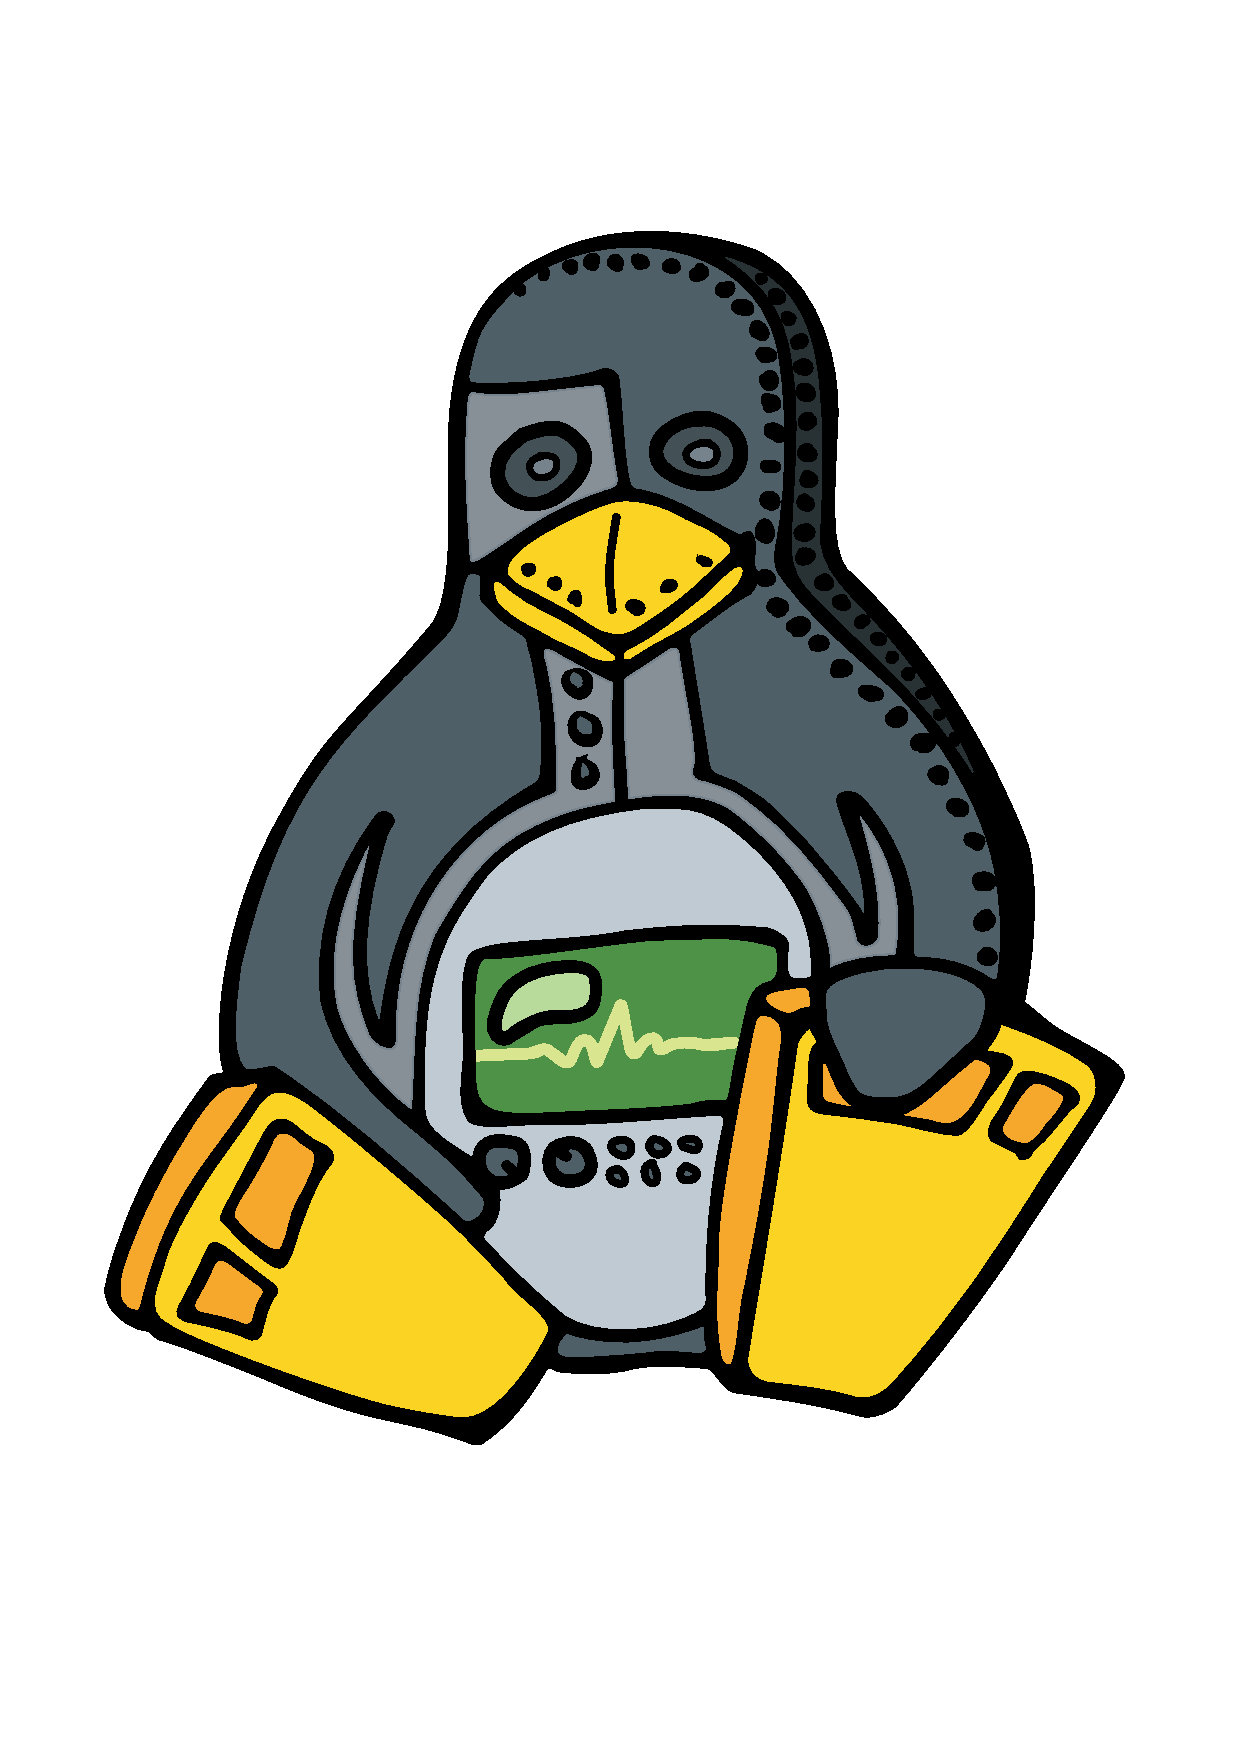
\includegraphics[height=3cm]{figures/ohr_logo.pdf}
  \label{fig:ohr_logo}
\end{figure}

% Generate the title
\maketitle

% Document abstract
\begin{abstract}
This document, blabla...
\end{abstract}


% Revision history
\newpage
\begin{tabularx}{1.0\textwidth}{| c | c | l | X |}
\hline
Revision & Date & Author &  Comments\\
\hline
0.1 & 07.02.2012 & Matthieu CATTIN & Initial revision\\
\hline
\end{tabularx}

% Insert a table of content
\newpage
\tableofcontents

% Start sections on a new page
\newpage

%===============================================================================
\section{Overview}
Here's an overview of the fmcadc100m14b4cha board...

\begin{figure}[h!]
  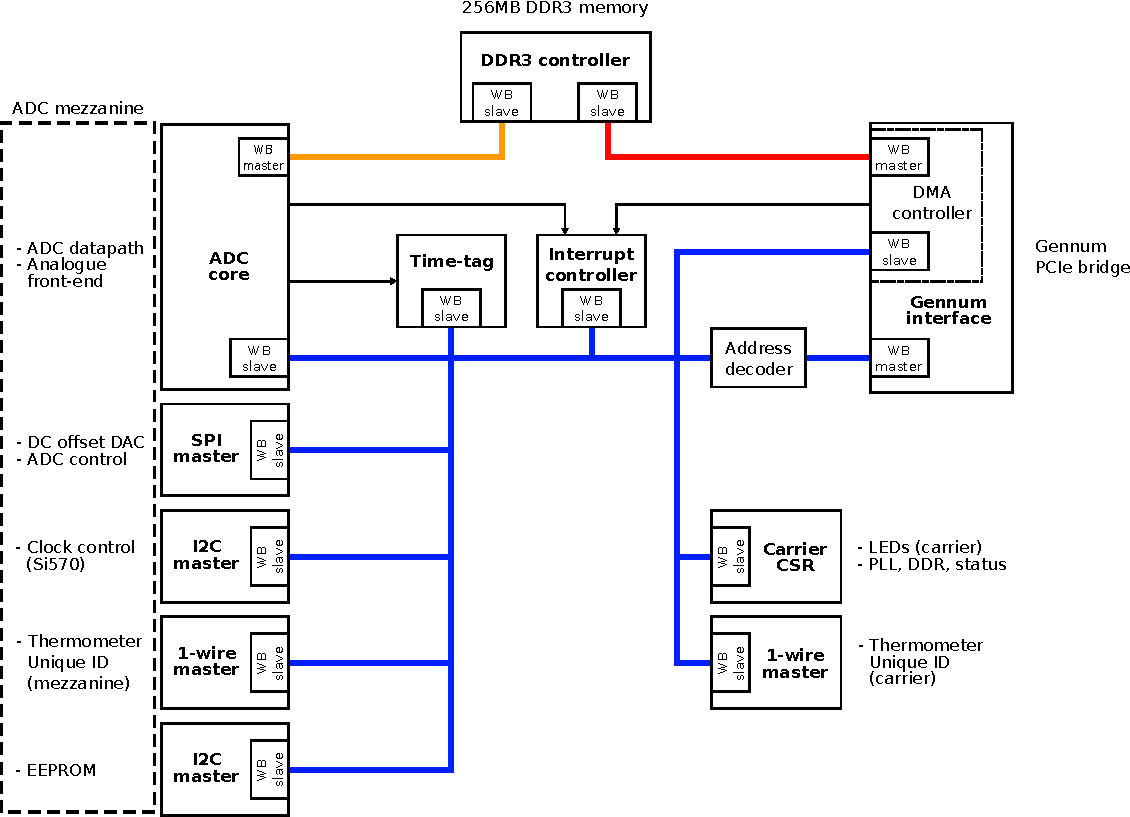
\includegraphics[width=\textwidth]{figures/firmware_arch.pdf}
  \caption{FPGA firmware architecture.}
  \label{fig:firmware_arch}
\end{figure}

%===============================================================================
\section{Settings}


\subsection{Trigger}
Software and/or hardware trigger. Internal or external hardware trigger, polarity selection.
Optional additional delay on the final trigger (in sampling clock ticks).

\begin{figure}[h!]
  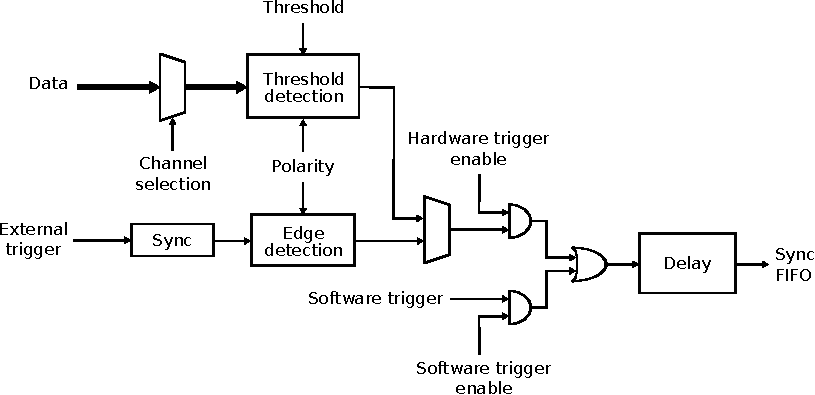
\includegraphics[width=\textwidth]{figures/trigger_unit.pdf}
  \caption{Trigger unit details.}
  \label{fig:trigger_unit}
\end{figure}


\subsection{Input ranges}
Three input ranges, optional input 50ohms termination.
Calibration input configuration.


\subsection{Input offset}

\begin{equation}\label{dac_digital2volts}
V\subscript{dac} = V\subscript{ref} \cdot \frac{32768 \cdot D\subscript{dac}}{32768} \\
\end{equation}
where:
\begin{equation}
V\subscript{ref} = 5 [Volts]
\end{equation}


\begin{equation}\label{in_dac_offset}
V\subscript{out} = V\subscript{in} - (gain\subscript{dac} \cdot V\subscript{dac} + offset\subscript{dac})
\end{equation}


\subsection{Time-stamping}



%===============================================================================
\section{Acquisition}

\begin{figure}[h!]
  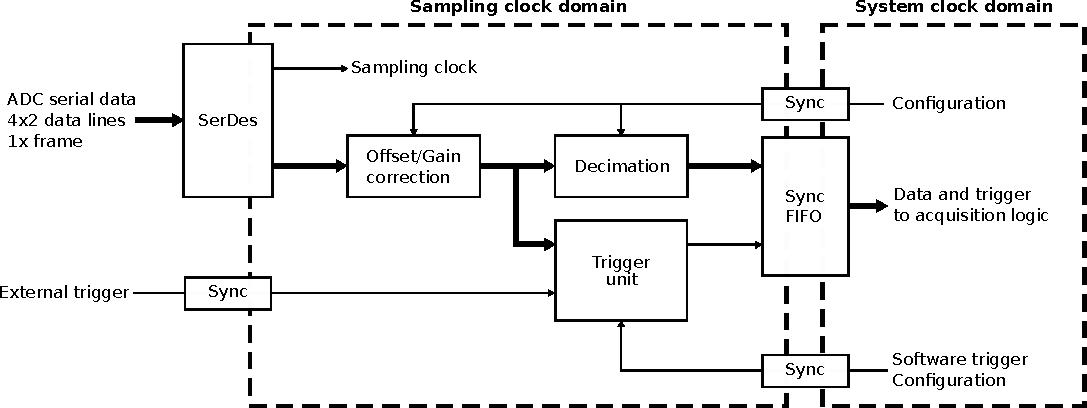
\includegraphics[width=\textwidth]{figures/adc_core_fs_clk.pdf}
  \caption{ADC core, sampling clock domain.}
  \label{fig:adc_core_fs_clk}
\end{figure}

\begin{figure}[h!]
  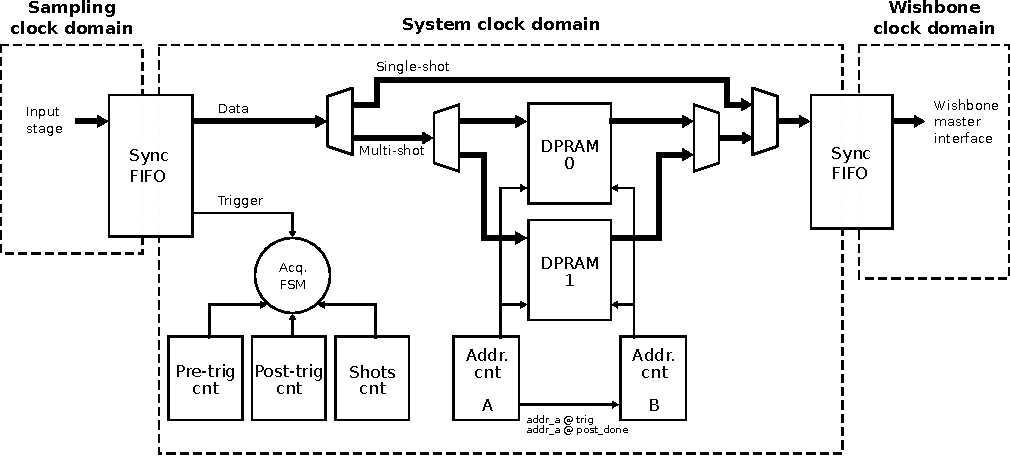
\includegraphics[width=\textwidth]{figures/adc_core_sys_clk.pdf}
  \caption{ADC core, system clock domain.}
  \label{fig:adc_core_sys_clk}
\end{figure}

\begin{itemize}

\item Single shot mode
  \begin{itemize}
  \item State machine
  \item Memory managment
  \item ...
  \end{itemize}

\item Multi-shot mode
  \begin{itemize}
  \item State machine
  \item Memory managment
  \item ...
  \end{itemize}
\end{itemize}




%===============================================================================
\newpage
\section{Calibration}

The calibration is done once during the prodoction tests.
It can be repeated afterwards with the production test suite (PTS) and the corresponding testbench.
The calibration process gives four values per channel and per input range:
ADC gain correction, ADC offset correction, DAC gain correction and DAC offset correction.
The temperature during the calibration process is also measured.
All the calibration values are stored in the FmcAdc100m14b4cha EEPROM.
The EEPROM holds a sdbfs\footnote{http://www.ohwr.org/attachments/download/1594/sdbfs-2012-09-19.pdf} file system.
In addition to the calibration values, the EEPROM also contains mandatory IPMI\footnote{Platform Management FRU Information Storage Definition v1.0} 
records described in the FMC Standard VITA 57.1 (see table \ref{tab:eeprom_sdbfs} for mapping).

\begin{table}[ht]
  \centering
  \begin{tabularx}{\textwidth}{| l | l | l | X |}
    \hline
    \textbf{Byte offset} & \textbf{File name}  & \textbf{File Type} & \textbf{Description} \\
    \hline
    0x0 & ipmi.sdb & binary & IPMI records \\
    \hline
    0x100 & calibration.sdb & binary & Calibration values \\
    \hline
    0x1000 & . & binary & Directory \\
    & & & vendor = 0xCE42 \\
    & & & device = 0xC5BE045E \\
    \hline
  \end{tabularx}
  \caption{EEPROM sdbfs}
  \label{tab:eeprom_sdbfs}
\end{table}

Note that the vendor value 0xCE42 corresponds to CERN. While the device value 0xC5BE045E corresponds to the first 32-bit of the md5 sum of "fmc-adc-100m14b4cha".

Tables \ref{tab:adc_calibr_data_eeprom} and \ref{tab:dac_calibr_data_eeprom} shows the calibration data types and the arrangement in the binary file.
The first column "Byte offset" represents the offset within the binary file.

\begin{table}[ht]
  \centering
  \begin{tabularx}{\textwidth}{| >{\centering}p{1.1cm} | >{\centering}p{1.2cm} | l | X |}
    \hline
    \multicolumn{4}{|c|}{\textbf{ADC correction values}} \\ \hline
    \textbf{Byte offset} & \textbf{Input range}  & \textbf{Description} & \textbf{Type} \\ \hline
    0 & 10V & Offset correction channel 1 & 16-bit signed \\
    2 & & Offset correction channel 2 & 16-bit signed \\
    4 & & Offset correction channel 3 & 16-bit signed \\
    6 & & Offset correction channel 4 & 16-bit signed \\
    \cline{3-4}
    8 & & Gain correction channel 1 & 16-bit unsigned \\
    10 & & Gain correction channel 2 & 16-bit unsigned \\
    12 & & Gain correction channel 3 & 16-bit unsigned \\
    14 & & Gain correction channel 4 & 16-bit unsigned \\
    \cline{3-4}
    16 & & Temperature & 16-bit unsigned * 0.01$^\circ$C \\
    \hline
    18 & 1V & Offset correction channel 1 & 16-bit signed \\
    20 & & Offset correction channel 2 & 16-bit signed \\
    22 & & Offset correction channel 3 & 16-bit signed \\
    24 & & Offset correction channel 4 & 16-bit signed \\
    \cline{3-4}
    26 & & Gain correction channel 1 & 16-bit unsigned \\
    28 & & Gain correction channel 2 & 16-bit unsigned \\
    30 & & Gain correction channel 3 & 16-bit unsigned \\
    32 & & Gain correction channel 4 & 16-bit unsigned \\
    \cline{3-4}
    34 & & Temperature & 16-bit unsigned * 0.01$^\circ$C \\
    \hline
    36 & 100mV & Offset correction channel 1 & 16-bit signed \\
    38 & & Offset correction channel 2 & 16-bit signed \\
    40 & & Offset correction channel 3 & 16-bit signed \\
    42 & & Offset correction channel 4 & 16-bit signed \\
    \cline{3-4}
    44 & & Gain correction channel 1 & 16-bit unsigned \\
    46 & & Gain correction channel 2 & 16-bit unsigned \\
    48 & & Gain correction channel 3 & 16-bit unsigned \\
    50 & & Gain correction channel 4 & 16-bit unsigned \\
    \cline{3-4}
    52 & & Temperature & 16-bit unsigned * 0.01$^\circ$C \\
    \hline
  \end{tabularx}
  \caption{ADC calibration data}
  \label{tab:adc_calibr_data_eeprom}
\end{table}

\begin{table}[ht]
  \centering
  \begin{tabularx}{\textwidth}{| >{\centering}p{1.1cm} | >{\centering}p{1.2cm} | l | X |}
    \hline
    \multicolumn{4}{|c|}{\textbf{DAC correction values}} \\ \hline
    \textbf{Byte offset} & \textbf{Input range}  & \textbf{Description} & \textbf{Type} \\ \hline
    54 & 10V & Offset correction channel 1 & 16-bit signed \\
    56 & & Offset correction channel 2 & 16-bit signed \\
    58 & & Offset correction channel 3 & 16-bit signed \\
    60 & & Offset correction channel 4 & 16-bit signed \\
    \cline{3-4}
    62 & & Gain correction channel 1 & 16-bit unsigned \\
    64 & & Gain correction channel 2 & 16-bit unsigned \\
    66 & & Gain correction channel 3 & 16-bit unsigned \\
    68 & & Gain correction channel 4 & 16-bit unsigned \\
    \cline{3-4}
    70 & & Temperature & 16-bit unsigned * 0.01$^\circ$C \\
    \hline
    72 & 1V & Offset correction channel 1 & 16-bit signed \\
    74 & & Offset correction channel 2 & 16-bit signed \\
    76 & & Offset correction channel 3 & 16-bit signed \\
    78 & & Offset correction channel 4 & 16-bit signed \\
    \cline{3-4}
    80 & & Gain correction channel 1 & 16-bit unsigned \\
    82 & & Gain correction channel 2 & 16-bit unsigned \\
    84 & & Gain correction channel 3 & 16-bit unsigned \\
    86 & & Gain correction channel 4 & 16-bit unsigned \\
    \cline{3-4}
    88 & & Temperature & 16-bit unsigned * 0.01$^\circ$C \\
    \hline
    90 & 100mV & Offset correction channel 1 & 16-bit signed \\
    92 & & Offset correction channel 2 & 16-bit signed \\
    94 & & Offset correction channel 3 & 16-bit signed \\
    96 & & Offset correction channel 4 & 16-bit signed \\
    \cline{3-4}
    98 & & Gain correction channel 1 & 16-bit unsigned \\
    100 & & Gain correction channel 2 & 16-bit unsigned \\
    102 & & Gain correction channel 3 & 16-bit unsigned \\
    104 & & Gain correction channel 4 & 16-bit unsigned \\
    \cline{3-4}
    106 & & Temperature & 16-bit unsigned * 0.01$^\circ$C \\
    \hline
  \end{tabularx}
  \caption{DAC calibration data}
  \label{tab:dac_calibr_data_eeprom}
\end{table}

Two registers per channel are implemented in the FPGA for ADC gain and offset correction.
When an input range is selected, the corresponding gain/offset correction values must be loaded from the EEPROM to those registers.

As the DAC value is set once before an acquisition, there is no need to implement the gain and offset correction in the FPGA.
Therefore gain and offset correction must be applied to the DAC value by the software.

Below is the pseudo-code to calculate the DAC corrected value, applying gain and offset correction:
\begin{verbatim}
c_val = ((((val-0x8000+offset) << 15) * gain) >> 30)+0x8000
\end{verbatim}
where:
\begin{verbatim}
c_val  = corrected value to write to DAC
val    = value from user
offset = DAC offset calibration value from EEPROM
gain   = DAC gain calibration value from EEPROM
\end{verbatim}







\end{document}
